\documentclass[format=acmsmall,review=false, screen=true, authorversion=true]{acmart}
%,review=false, screen=true, authorversion=true]

\usepackage{booktabs} % For formal tables
\usepackage{amsmath}
\usepackage[ruled]{algorithm2e} % For algorithms
\renewcommand{\algorithmcfname}{ALGORITHM}
\SetAlFnt{\small}
\SetAlCapFnt{\small}
\SetAlCapNameFnt{\small}
\SetAlCapHSkip{0pt}
\IncMargin{-\parindent}



% Copyright
%\setcopyright{acmcopyright}
\setcopyright{acmlicensed}
%\setcopyright{rightsretained}
%\setcopyright{usgov}
%\setcopyright{usgovmixed}
%\setcopyright{cagov}
%\setcopyright{cagovmixed}



% Document starts
\begin{document}
% Title portion. Note the short title for running heads 
\title{IE590 Project}  
\author{Huiting Su}
\maketitle


I am aware of, and understand, the Purdue Academic Misconduct Policies
and attest that this submitted work is solely my own. I accept any repercussions if found in violation.

\section{Synopsis}
Gesture is an important part in human communication, and wearable devices have been used in many fields nowadays. A wearable device which can transfer gesture to electric current time series is developed by Ruoxing Wang, a PhD student of Purdue Industrial Engineering. 

Given the current data, we want to make the wearable device able to recognize different gestures. In this project, I collaborate with Ruoxing Wang. She provides raw experiment data, and I implement neural network algorithm to recognize the gesture. 

\section{Problem Description}
The goal in this project is mainly to distinguish between ``OK'' gesture and waving gesture. The electric current is shown in real time by the device while a person is using the wearable device. Examples of the current of two gestures is shown in fig.\ref{fig:ok1} and fig. \ref{fig:wave1}. 

The current data is available every 0.001 second, so we have a huge amount of data even only for a single gesture. As we want to recognize the gesture in real time, it is easier and makes more sense to recognize through image than processing the raw data.     

\begin{figure}[h]
\centering
\begin{minipage}{.49\textwidth}
  \centering
  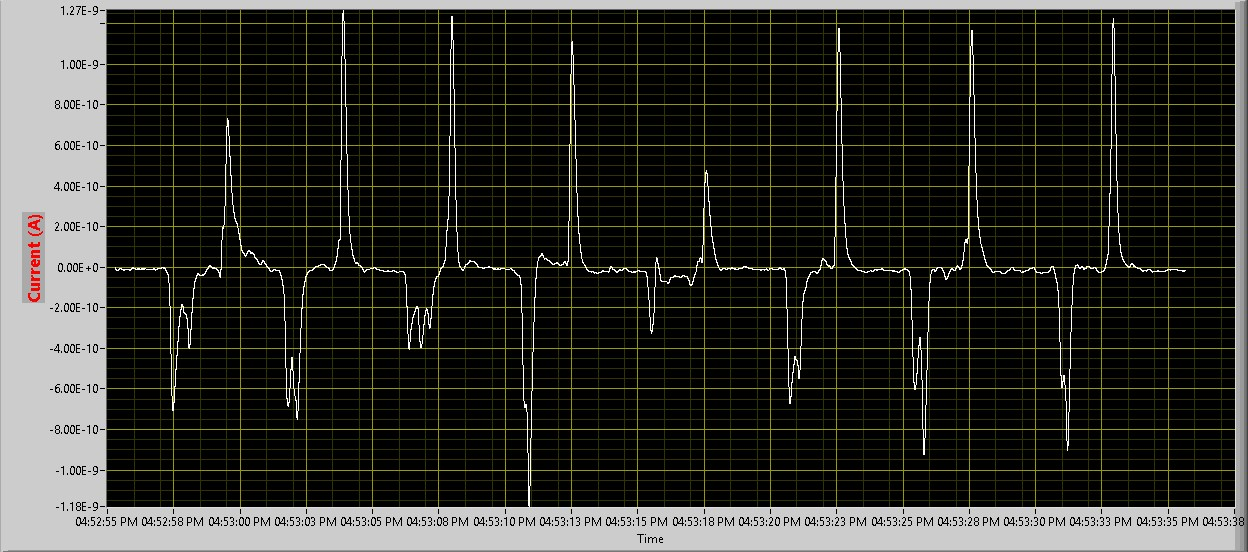
\includegraphics[width=.95\linewidth]{pok1}
  \captionof{figure}{Current of ``OK'' gesture}
  \label{fig:ok1}
\end{minipage}
\begin{minipage}{.49\textwidth}
  \centering
  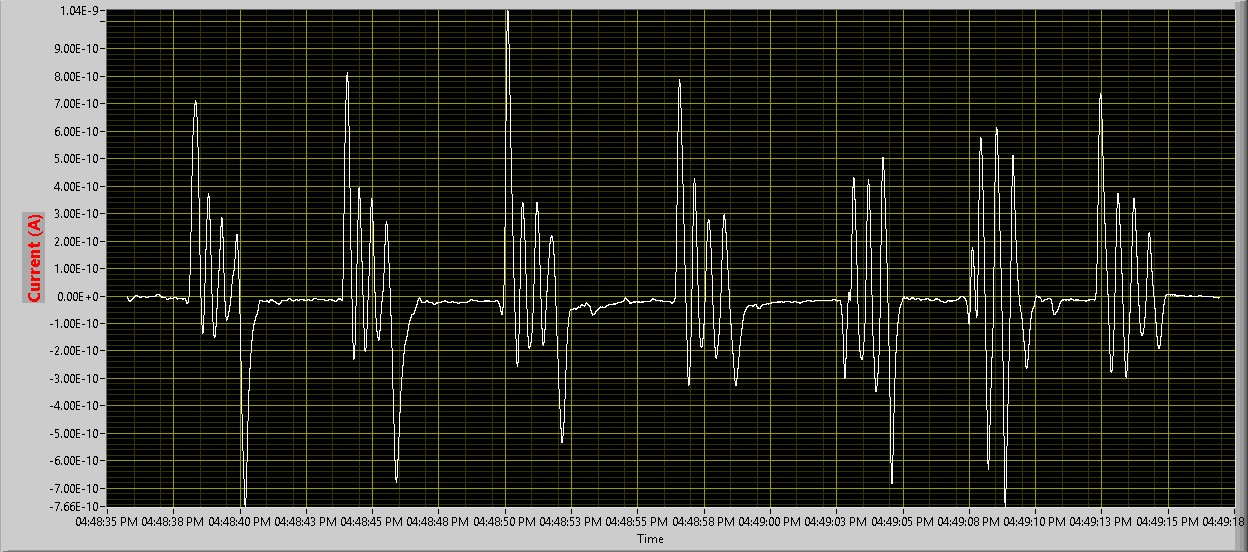
\includegraphics[width=.95\linewidth]{pwave1}
  \captionof{figure}{Current of waving gesture}
  \label{fig:wave1}
\end{minipage}
\end{figure}


\section{Data Processing}
The current data is seperated into single gestures manually, since the focus is the implementation of the artificial neural network. There are 41 current images in total, while 14 of them are ``OK'' gestures and 27 of them are waving gestures. Examples are shown in fig. \ref{fig:eg1} and fig. \ref{fig:eg2}.

\begin{figure}[h]
\centering
\begin{minipage}{.49\textwidth}
  \centering
  
\includegraphics[width=.1\linewidth]{ok1}
  \captionof{figure}{Splitted $28 \times 28$ pixels OK image}
  \label{fig:eg1}
\end{minipage}
\begin{minipage}{.49\textwidth}
  \centering
  
\includegraphics[width=.1\linewidth]{ok2}
  \captionof{figure}{Splitted $28 \times 28$ pixels OK image}
  \label{fig:eg2}
\end{minipage}
\end{figure}

The images are $28 \times 28$ pixels, then are transfered into grayscale flattened array. That is to say, every image is represented by a vector whose length is $28 \times 28$. The elements in the vector are scaled into $[0, 1]$, which represent the amount of light in the corresponding pixels. When the element equals to 0, then the pixel is black; on the other hand, if the element equals to 1, the pixel is white. 

Two different labels are assigned to the vectors: 0 for   ``OK'' gesture, and 1 for waving gesture. Randomly select 30 vetors to form the training data, and the remaining 11 vectors become the testing data.
 
 
\section{Ordinary Least Squares}
First try with ordinary least square linear regression. Define the pixels as input variables and the gesture label as response. Fit a model using the training set, then predict the response of the model. 7 predictions out of 11 are correct, which yeilds a correct rate of 0.636. This method is not so promising. 

\section{Implementation of Neural Network}
Build a neural network with mxnet package in R. The symbolic model contains two convolutional layers and two fully connected layers.  After training the network, test it on the test set, and the neural network achieves a correct rate of 100\%.  

\subsection{Cross Validation}
 The previous result is only based on one set of training data and testing data. In order to know how well the algorithm performs on other sets of data, we can use cross validation to evaluate the performance of the algorithm. 
 
A k-fold Cross Validation is a process of spliting train-test data, performing training and testing, calculating the prediction error, and repeat k times. Then the performance of algorithm can be evaluated by taking the average of k prediction errors. 

\subsection{Parameter Tuning}
The result of initial test looks good, but we still need to tune the parameters in neural network to achive satisfiable results. The parameters we want to tune are described respectively. 
\subsubsection{Learning rate}
The learning rate is one of the most important hyper-parameters to tune for training deep neural networks. In a easy way to understand, the learning rate is how quickly the neural nextwork change the inference from previous learning to accept new belief. 

If the learning rate is too high, which means the network also change belief when it is encountered new data, it takes a long time to train it. If the learning rate is too low, it may stick to the conclusions it made from the initial data. We want to tune the network to find a suitable learning rate, which can let it converge to meaningfule result quickly enough.   

\subsubsection{momentum}
When minimizing the error function, the gradient descent method is used. As there is no evidence that the function is convex, the algorithm can be trapped in a local optima. Momentum is a step size which helps the algorithm step out local optima.

\subsubsection{Dropout}
Dropout is a technique for reducing overfitting in the trainning process. It prevents complex co-adaptations on training set. We can assign the dropout to be ``training'', which means it only performs dropout during training, or ``always'', which also performs dropout in testing. Here dropout is assigned to be ``training''. 

\subsubsection{Activation Function}
Activation function contain 'relu', 'sigmoid', 'softrelu' and 'tanh'. Sigmoid function is the most commonly used function, which gives value very close to 0 when x is very negative, close to 1 when very positive, and close to linear in [-1, 1]. Relu function gives 0 value when x is negative, and as it is when x is positive. In order to be consistent with the algorithm used previously, we choose 'tanh' function for activation.  

\subsection{Experiment}
An experiment is conducted using package caret in R. With this package we can perform cross validation and tune parameters. A 10-fold cross validation is used in this case. The result is shown in table .\ref{tab:tune}. The final values used for the model were learning rate =0.01, momentum = 0.9, dropout = training and activation
 = tanh. As we can see, with this parameter combination, the algorithm achieves accuracy of 0.855, which is high. 
 
\begin{table}[h]
\caption{Parameter Tuning Result}
\label{tab:tune}
\begin{center}
\begin{tabular}{c c c c}
  \hline
learning.rate  &momentum  &Accuracy    &Kappa\\       
  0.001          &0.0       &0.718  &0.280\\
  0.001          &0.9       &0.763  &0.400\\
  0.010          &0.0       &0.803  &0.516\\
  0.010          &0.9       &0.855  &0.650\\
  0.100          &0.0       &0.722  &0.179\\
  0.100          &0.9       &0.663  &0.000\\
\hline
\end{tabular}
\end{center}
\end{table}

For further experiment details, please refer to the R markdown files.

\section{conclusion and Future Work}

\begin{enumerate}
\item Neural network has satisfiable performance in image classification;
\item More gestures data like ``1'', ``6'', ``0'' will be added to the training set;
\item A real time classification program will be devised. 
\end{enumerate}



%\bibliographystyle{ACM-Reference-Format}
%\bibliography{bibliography4} 
\end{document}